\documentclass[10pt]{beamer}
\usepackage[utf8]{inputenc}
\usepackage[T1]{fontenc}
\usetheme{metropolis}
\usepackage{booktabs}
\usepackage[scale=2]{ccicons}
\usepackage{pgfplots}
\usepgfplotslibrary{dateplot}
\usepackage{xspace}
\usepackage{pbox}

% a few macros
\newcommand{\bi}{\begin{itemize}}
\newcommand{\ei}{\end{itemize}}
\newcommand{\be}{\begin{enumerate}}
\newcommand{\ee}{\end{enumerate}}
\newcommand{\ig}{\includegraphics}
\definecolor{hilight}{RGB}{235,129,27}
\definecolor{vhilight}{RGB}{235,129,27}
\definecolor{title}{RGB}{107,174,214}
\definecolor{subtitle}{RGB}{102,255,204}

% title info
\title{Graphs}
\subtitle{Unweighted Graphs}
\author{Bjarki Ágúst Guðmundsson\\ Tómas Ken Magnússon}
\institute{\href{http://ru.is/td}{School of Computer Science} \\[2pt] \href{http://ru.is}{Reykjavík University}}
\titlegraphic{\hfill\includegraphics[height=0.6cm]{kattis}}
\date{\textbf{Árangursrík forritun og lausn verkefna}}

% Tikz
\usepackage{tikz}
\usetikzlibrary{arrows,shapes}

% Minted
\usepackage{minted}
\usemintedstyle{manni}
\newminted{cpp}{fontsize=\footnotesize}

% Graph styles
\tikzstyle{vertex}=[circle,fill=black!50,minimum size=15pt,inner sep=0pt, font=\small]
\tikzstyle{selected vertex} = [vertex, fill=red!24]
\tikzstyle{edge} = [draw,thick,-]
\tikzstyle{dedge} = [draw,thick,->]
\tikzstyle{weight} = [font=\scriptsize,pos=0.5]
\tikzstyle{selected edge} = [draw,line width=2pt,-,red!50]
\tikzstyle{ignored edge} = [draw,line width=5pt,-,black!20]

\tikzset{
  treenode/.style = {align=center, inner sep=0pt, text centered,
    font=\sffamily},
  vertex/.style = {treenode, circle, black, font=\sffamily\bfseries\tiny, draw=black, text width=1.8em},% arbre rouge noir, noeud noir
  rvertex/.style = {treenode, circle, black, font=\sffamily\bfseries\tiny, draw=red, text width=1.8em},% arbre rouge noir, noeud noir
}

\begin{document}
\maketitle

\begin{frame}{Today we're going to cover}
    \vspace{10pt}
    \bi
        \item Graph basics
        \item Graph representation (recap)
        \item Depth-first search
        % \item Flood-fill
        \item Connected components
        \item DFS tree
        \item Bridges
        \item Strongly connected components
        \item Topological sort
        \item Breadth-first search
        \item Shortest paths in unweighted graphs
    \ei
\end{frame}


\begin{frame}{What is a graph?}
    \begin{columns}[T]
        \begin{column}{.6\textwidth}
            \bi
                \onslide<2->{
                    \item Vertices
                        \bi
                            \item Road intersections
                            \item Computers
                            \item Floors in a house
                            \item Objects
                        \ei
                }
                \onslide<3->{
                    \item Edges
                        \bi
                            \item Roads
                            \item Ethernet cables
                            \item Stairs or elevators
                            \item Relation between objects
                        \ei
                }
            \ei
        \end{column}%
        \hfill%
        \begin{column}{.6\textwidth}
            \begin{figure}
                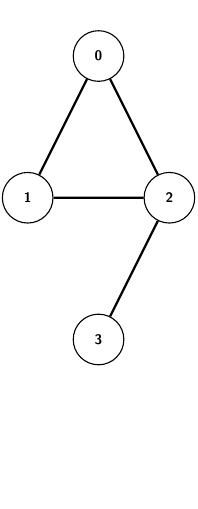
\begin{tikzpicture}[scale=1.8,auto,swap]
                    \onslide<2->{
                        \node[vertex] (0) at (0.5,3) {0};
                        \node[vertex] (1) at (0,2) {1};
                        \node[vertex] (2) at (1,2) {2};
                        \node[vertex] (3) at (0.5,1) {3};
                    }

                    \onslide<3->{
                        \path[edge] (0) -- (1);
                        \path[edge] (0) -- (2);
                        \path[edge] (1) -- (2);
                        \path[edge] (2) -- (3);
                    }
                    \pgfresetboundingbox
                    \path [use as bounding box] (0,0) rectangle (1,3.2);
                \end{tikzpicture}
            \end{figure}
        \end{column}%
    \end{columns}
\end{frame}

\begin{frame}{Types of edges}
    \begin{columns}[T]
        \begin{column}{.6\textwidth}
            \bi
                \item \color<1>{hilight}{Unweighted} \onslide<2->{or \color<2>{hilight} Weighted}
                \onslide<3->{\item \color<3>{hilight} Undirected} \onslide<4->{or \color<4,5>{hilight} Directed}
            \ei
        \end{column}%
        \hfill%
        \begin{column}{.6\textwidth}
            \begin{figure}
                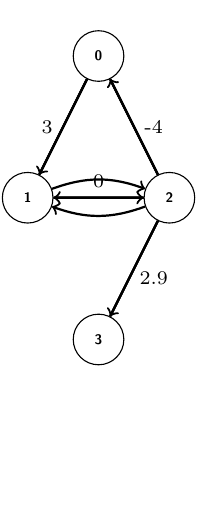
\begin{tikzpicture}[scale=1.8,auto,swap]
                    \node[vertex] (0) at (0.5,3) {0};
                    \node[vertex] (1) at (0,2) {1};
                    \node[vertex] (2) at (1,2) {2};
                    \node[vertex] (3) at (0.5,1) {3};

                    \onslide<1,3>{
                        \path[edge] (0) -- (1);
                        \path[edge] (0) -- (2);
                        \path[edge] (1) -- (2);
                        \path[edge] (2) -- (3);
                    }

                    \onslide<2>{
                        \path[edge] (0) -- node[weight,left] {3} (1);
                        \path[edge] (0) -- node[weight,right] {-4} (2);
                        \path[edge] (1) -- node[weight,above] {0} (2);
                        \path[edge] (2) -- node[weight,right,pos=0.6] {2.9} (3);
                    }

                    \onslide<4-5>{
                        \path[dedge] (0) -- (1);
                        \path[dedge] (2) -- (0);
                        \onslide<4>{
                            \path[dedge] (1) -- (2);
                            \path[dedge] (2) -- (1);
                        }
                        \onslide<5>{
                            \path[dedge] (1) edge[bend left=20] (2);
                            \path[dedge] (2) edge[bend left=20] (1);
                        }
                        \path[dedge] (2) -- (3);
                    }

                    \pgfresetboundingbox
                    \path [use as bounding box] (0,0) rectangle (1,3.2);
                \end{tikzpicture}
            \end{figure}
        \end{column}%
    \end{columns}
\end{frame}


\begin{frame}{Multigraphs}
    \begin{columns}[T]
        \begin{column}{.6\textwidth}
            \bi
                \onslide<2->{\item \color<2>{hilight} Multiple edges}
                \onslide<3->{\item \color<3>{hilight} Self-loops}
            \ei
        \end{column}%
        \hfill%
        \begin{column}{.6\textwidth}
            \begin{figure}
                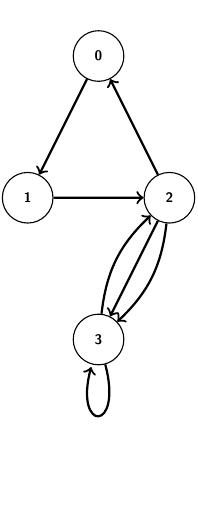
\begin{tikzpicture}[scale=1.8,auto,swap]
                    \node[vertex] (0) at (0.5,3) {0};
                    \node[vertex] (1) at (0,2) {1};
                    \node[vertex] (2) at (1,2) {2};
                    \node[vertex] (3) at (0.5,1) {3};

                    \path[dedge] (0) -- (1);
                    \path[dedge] (2) -- (0);
                    \path[dedge] (2) -- (3);
                    \path[dedge] (1) -- (2);

                    \onslide<2>{
                        \path[dedge] (2) edge[bend left=20] (3);
                        \path[dedge] (3) edge[bend left=20] (2);
                    }

                    \onslide<3>{
                        \path[dedge] (3) edge[loop below] (3);
                    }

                    \pgfresetboundingbox
                    \path [use as bounding box] (0,0) rectangle (1,3.2);
                \end{tikzpicture}
            \end{figure}
        \end{column}%
    \end{columns}
\end{frame}


\begin{frame}[fragile]{Adjacency list}

    \begin{columns}[T]
        \begin{column}{.4\textwidth}
            \begin{minted}{cpp}
0: 1, 2
1: 0, 2
2: 0, 1, 3
3: 2

vector<int> adj[4];
adj[0].push_back(1);
adj[0].push_back(2);
adj[1].push_back(0);
adj[1].push_back(2);
adj[2].push_back(0);
adj[2].push_back(1);
adj[2].push_back(3);
adj[3].push_back(2);
            \end{minted}
        \end{column}%
        \hfill%
        \begin{column}{.4\textwidth}
            \begin{figure}
                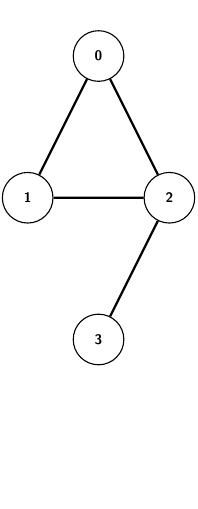
\begin{tikzpicture}[scale=1.8,auto,swap]
                    \node[vertex] (0) at (0.5,3) {0};
                    \node[vertex] (1) at (0,2) {1};
                    \node[vertex] (2) at (1,2) {2};
                    \node[vertex] (3) at (0.5,1) {3};

                    \path[edge] (0) -- (1);
                    \path[edge] (2) -- (0);
                    \path[edge] (2) -- (3);
                    \path[edge] (1) -- (2);

                    \pgfresetboundingbox
                    \path [use as bounding box] (0,0) rectangle (1,3.2);
                \end{tikzpicture}
            \end{figure}
        \end{column}%
    \end{columns}
\end{frame}


\begin{frame}[fragile]{Adjacency list (directed)}

    \begin{columns}[T]
        \begin{column}{.4\textwidth}
            \begin{minted}{cpp}
0: 1
1: 2
2: 0, 1, 3
3:

vector<int> adj[4];
adj[0].push_back(1);
adj[1].push_back(2);
adj[2].push_back(0);
adj[2].push_back(1);
adj[2].push_back(3);
            \end{minted}
        \end{column}%
        \hfill%
        \begin{column}{.4\textwidth}
            \begin{figure}
                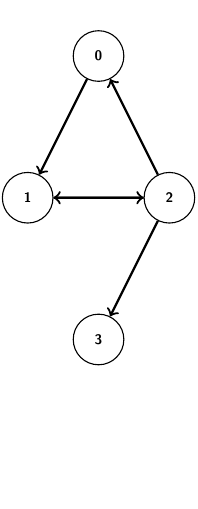
\begin{tikzpicture}[scale=1.8,auto,swap]
                    \node[vertex] (0) at (0.5,3) {0};
                    \node[vertex] (1) at (0,2) {1};
                    \node[vertex] (2) at (1,2) {2};
                    \node[vertex] (3) at (0.5,1) {3};

                    \path[dedge] (0) -- (1);
                    \path[dedge] (2) -- (0);
                    \path[dedge] (2) -- (3);
                    \path[dedge] (1) -- (2);
                    \path[dedge] (2) -- (1);

                    \pgfresetboundingbox
                    \path [use as bounding box] (0,0) rectangle (1,3.2);
                \end{tikzpicture}
            \end{figure}
        \end{column}%
    \end{columns}
\end{frame}



\begin{frame}[fragile]{Vertex properties (undirected graph)}
    \begin{columns}[T]
        \begin{column}{.6\textwidth}
            \vspace{20pt}
            \bi
                \item Degree of a vertex
                    \bi
                        \item Number of adjacent edges
                        \item Number of adjacent vertices
                    \ei
% 
%                 \item In terms of our adjacency list:
%                     \begin{minted}{cpp}
%   adj[v].size()
%                     \end{minted}
%                     \vspace{20pt}

                \onslide<3->{
                    \item Handshaking lemma
                        $$ \sum_{v\in V} \mathrm{deg}(v) = 2|E| $$
                    \onslide<4->{
                        $$
                            2 + 2 + 3 + 1 = 2\times 4
                        $$
                    }
                }
            \ei
        \end{column}%
        \hfill%
        \begin{column}{.6\textwidth}
            \begin{figure}
                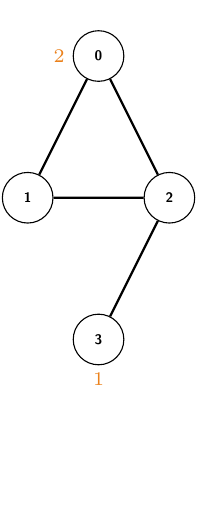
\begin{tikzpicture}[scale=1.8,auto,swap]
                    \node[vertex] (0) at (0.5,3) {0};
                    \node[vertex] (1) at (0,2) {1};
                    \node[vertex] (2) at (1,2) {2};
                    \node[vertex] (3) at (0.5,1) {3};

                    \path[edge] (0) -- (1);
                    \path[edge] (2) -- (0);
                    \path[edge] (2) -- (3);
                    \path[edge] (1) -- (2);

                    \onslide<2->{
                        \node[font=\scriptsize,shift={(-0.5,0)},color=vhilight] at (0) {2};
                        \node[font=\scriptsize,shift={(-0.5,0)},color=vhilight] at (1) {2};
                        \node[font=\scriptsize,shift={(0.5,0)},color=vhilight] at (2) {3};
                        \node[font=\scriptsize,shift={(0,-0.5)},color=vhilight] at (3) {1};
                    }
                    \pgfresetboundingbox
                    \path [use as bounding box] (0,0) rectangle (1,3.2);
                \end{tikzpicture}
            \end{figure}
        \end{column}%
    \end{columns}
\end{frame}


\begin{frame}[fragile]{Vertex properties (undirected graph)}

    \begin{columns}[T]
        \begin{column}{.4\textwidth}
            \begin{minted}{cpp}
0: 1, 2
1: 0, 2
2: 0, 1, 3
3: 2

adj[0].size() // 2
adj[1].size() // 2
adj[2].size() // 3
adj[3].size() // 1
            \end{minted}
        \end{column}%
        \hfill%
        \begin{column}{.4\textwidth}
            \begin{figure}
                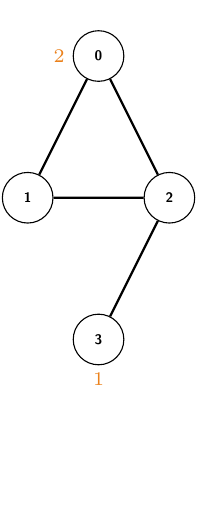
\begin{tikzpicture}[scale=1.8,auto,swap]
                    \node[vertex] (0) at (0.5,3) {0};
                    \node[vertex] (1) at (0,2) {1};
                    \node[vertex] (2) at (1,2) {2};
                    \node[vertex] (3) at (0.5,1) {3};

                    \path[edge] (0) -- (1);
                    \path[edge] (2) -- (0);
                    \path[edge] (2) -- (3);
                    \path[edge] (1) -- (2);

                    \node[font=\scriptsize,shift={(-0.5,0)},color=vhilight] at (0) {2};
                    \node[font=\scriptsize,shift={(-0.5,0)},color=vhilight] at (1) {2};
                    \node[font=\scriptsize,shift={(0.5,0)},color=vhilight] at (2) {3};
                    \node[font=\scriptsize,shift={(0,-0.5)},color=vhilight] at (3) {1};

                    \pgfresetboundingbox
                    \path [use as bounding box] (0,0) rectangle (1,3.2);
                \end{tikzpicture}
            \end{figure}
        \end{column}%
    \end{columns}
\end{frame}


\begin{frame}{Vertex properties (directed graph)}
    \begin{columns}[T]
        \begin{column}{.6\textwidth}
            \bi
                \onslide<1->{
                    \item Outdegree of a vertex
                        \bi
                            \item Number of outgoing edges
                        \ei
                }
                \onslide<3->{
                    \item Indegree of a vertex
                        \bi
                            \item Number of incoming edges
                        \ei
                }
            \ei
        \end{column}%
        \hfill%
        \begin{column}{.6\textwidth}
            \begin{figure}
                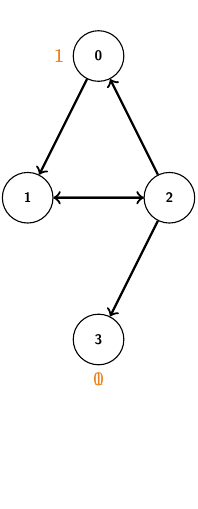
\begin{tikzpicture}[scale=1.8,auto,swap]
                    \node[vertex] (0) at (0.5,3) {0};
                    \node[vertex] (1) at (0,2) {1};
                    \node[vertex] (2) at (1,2) {2};
                    \node[vertex] (3) at (0.5,1) {3};

                    \path[dedge] (0) -- (1);
                    \path[dedge] (2) -- (0);
                    \path[dedge] (2) -- (3);
                    \path[dedge] (1) -- (2);
                    \path[dedge] (2) -- (1);

                    \onslide<2,6>{
                        \node[font=\scriptsize,shift={(-0.5,0)},color=vhilight] at (0) {1};
                        \node[font=\scriptsize,shift={(-0.5,0)},color=vhilight] at (1) {1};
                        \node[font=\scriptsize,shift={(0.5,0)},color=vhilight] at (2) {3};
                        \node[font=\scriptsize,shift={(0,-0.5)},color=vhilight] at (3) {0};
                    }

                    \onslide<4>{
                        \node[font=\scriptsize,shift={(-0.5,0)},color=vhilight] at (0) {1};
                        \node[font=\scriptsize,shift={(-0.5,0)},color=vhilight] at (1) {2};
                        \node[font=\scriptsize,shift={(0.5,0)},color=vhilight] at (2) {1};
                        \node[font=\scriptsize,shift={(0,-0.5)},color=vhilight] at (3) {1};
                    }




                    \pgfresetboundingbox
                    \path [use as bounding box] (0,0) rectangle (1,3.2);
                \end{tikzpicture}
            \end{figure}
        \end{column}%
    \end{columns}
\end{frame}


\begin{frame}[fragile]{Adjacency list (directed)}

    \begin{columns}[T]
        \begin{column}{.4\textwidth}
            \begin{minted}{cpp}
0: 1
1: 2
2: 0, 1, 3
3:

adj[0].size() // 1
adj[1].size() // 1
adj[2].size() // 3
adj[3].size() // 0
            \end{minted}
        \end{column}%
        \hfill%
        \begin{column}{.4\textwidth}
            \begin{figure}
                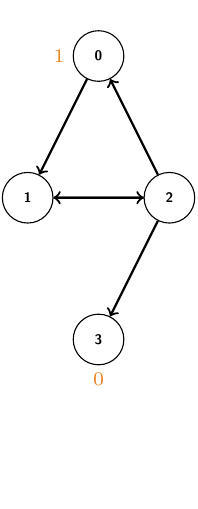
\begin{tikzpicture}[scale=1.8,auto,swap]
                    \node[vertex] (0) at (0.5,3) {0};
                    \node[vertex] (1) at (0,2) {1};
                    \node[vertex] (2) at (1,2) {2};
                    \node[vertex] (3) at (0.5,1) {3};

                    \path[dedge] (0) -- (1);
                    \path[dedge] (2) -- (0);
                    \path[dedge] (2) -- (3);
                    \path[dedge] (1) -- (2);
                    \path[dedge] (2) -- (1);

                    \node[font=\scriptsize,shift={(-0.5,0)},color=vhilight] at (0) {1};
                    \node[font=\scriptsize,shift={(-0.5,0)},color=vhilight] at (1) {1};
                    \node[font=\scriptsize,shift={(0.5,0)},color=vhilight] at (2) {3};
                    \node[font=\scriptsize,shift={(0,-0.5)},color=vhilight] at (3) {0};

                    \pgfresetboundingbox
                    \path [use as bounding box] (0,0) rectangle (1,3.2);
                \end{tikzpicture}
            \end{figure}
        \end{column}%
    \end{columns}
\end{frame}


\begin{frame}{Paths}
    \begin{columns}[T]
        \begin{column}{.6\textwidth}
            \bi
                \item Path / Walk / Trail:
                    $$
                        e_1 e_2 \ldots e_k
                    $$
                such that
                    $$ e_i \in E $$
                    $$ e_i = e_j \Rightarrow i = j $$
                    $$ \mathrm{to}(e_i) = \mathrm{from}(e_{i+1})$$
            \ei
        \end{column}%
        \hfill%
        \begin{column}{.6\textwidth}
            \begin{figure}
                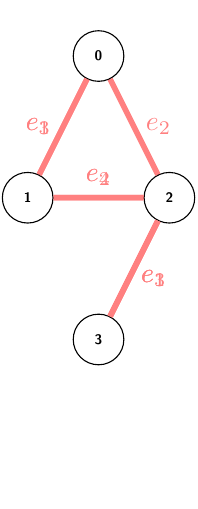
\begin{tikzpicture}[scale=1.8,auto,swap]
                    \node[vertex] (0) at (0.5,3) {0};
                    \node[vertex] (1) at (0,2) {1};
                    \node[vertex] (2) at (1,2) {2};
                    \node[vertex] (3) at (0.5,1) {3};

                    \onslide<1>{
                        \path[edge] (0) -- (1);
                        \path[edge] (2) -- (0);
                        \path[edge] (2) -- (3);
                        \path[edge] (1) -- (2);
                    }

                    \onslide<2>{
                        \path[selected edge] (0) -- node[left] {$e_1$} (1);
                        \path[edge] (2) -- (0);
                        \path[selected edge] (2) -- node[right,pos=0.6] {$e_3$} (3);
                        \path[selected edge] (1) -- node[above] {$e_2$} (2);
                    }

                    \onslide<3>{
                        \path[edge] (0) -- (1);
                        \path[edge] (2) -- (0);
                        \path[selected edge] (2) -- node[right,pos=0.6] {$e_1$} (3);
                        \path[edge] (1) -- (2);
                    }

                    \onslide<4>{
                        \path[selected edge] (0) -- node[left] {$e_3$} (1);
                        \path[selected edge] (2) -- node[right] {$e_2$} (0);
                        \path[selected edge] (2) -- node[right,pos=0.6] {$e_1$} (3);
                        \path[selected edge] (1) -- node[above] {$e_4$} (2);
                    }

                    \pgfresetboundingbox
                    \path [use as bounding box] (0,0) rectangle (1,3.2);
                \end{tikzpicture}
            \end{figure}
        \end{column}%
    \end{columns}
\end{frame}

\begin{frame}{Cycles}
    \begin{columns}[T]
        \begin{column}{.6\textwidth}
            \bi
                \item Cycle / Circuit / Tour:
                    $$
                        e_1 e_2 \ldots e_k
                    $$
                such that
                    $$ e_i \in E $$
                    $$ e_i = e_j \Rightarrow i = j $$
                    $$ \mathrm{to}(e_i) = \mathrm{from}(e_{i+1})$$
                    $$ \color<1>{vhilight}{\mathrm{from}(e_1) = \mathrm{to}(e_{k})} $$
            \ei
        \end{column}%
        \hfill%
        \begin{column}{.6\textwidth}
            \begin{figure}
                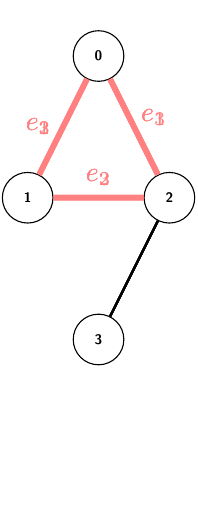
\begin{tikzpicture}[scale=1.8,auto,swap]
                    \node[vertex] (0) at (0.5,3) {0};
                    \node[vertex] (1) at (0,2) {1};
                    \node[vertex] (2) at (1,2) {2};
                    \node[vertex] (3) at (0.5,1) {3};

                    \onslide<1>{
                        \path[edge] (0) -- (1);
                        \path[edge] (2) -- (0);
                        \path[edge] (2) -- (3);
                        \path[edge] (1) -- (2);
                    }

                    \onslide<2>{
                        \path[selected edge] (0) -- node[left] {$e_1$} (1);
                        \path[selected edge] (2) -- node[right,pos=0.6] {$e_3$} (0);
                        \path[edge] (2) -- (3);
                        \path[selected edge] (1) -- node[above] {$e_2$} (2);
                    }

                    \onslide<3>{
                        \path[selected edge] (0) -- node[left] {$e_2$} (1);
                        \path[selected edge] (2) -- node[right,pos=0.6] {$e_1$} (0);
                        \path[edge] (2) -- (3);
                        \path[selected edge] (1) -- node[above] {$e_3$} (2);
                    }

                    \onslide<4>{
                        \path[selected edge] (0) -- node[left] {$e_3$} (1);
                        \path[selected edge] (2) -- node[right,pos=0.6] {$e_1$} (0);
                        \path[edge] (2) -- (3);
                        \path[selected edge] (1) -- node[above] {$e_2$} (2);
                    }

                    \pgfresetboundingbox
                    \path [use as bounding box] (0,0) rectangle (1,3.2);
                \end{tikzpicture}
            \end{figure}
        \end{column}%
    \end{columns}
\end{frame}

% TODO: Graph modeling

\begin{frame}{Depth-first search}
    \vspace{10pt}
    \bi
\item Given a graph (either directed or undirected) and two vertices $u$ and $v$, does there exist a path from $u$ to $v$?
\item Depth-first search is an algorithm for finding such a path, if one exists
    \vspace{10pt}

\item It traverses the graph in depth-first order, starting from the initial vertex $u$
\item We don't actually have to specify a $v$, since we can just let it visit all reachable vertices from $u$ (and still same time complexity)
    \vspace{10pt}
\item But what is the time complexity?
\item Each vertex is visited once, and each edge is traversed once
\item $O(n + m)$
    \ei
\end{frame}

\begin{frame}[fragile]{Depth-first search}
  \begin{figure}
    \begin{tikzpicture}[auto,swap]
      \node[vertex] (0) at (-0.3,2) {0};
      \node[vertex] (1) at (0.0,-0.5) {1};
      \node[vertex] (2) at (1.9,0.7) {2};
      \node[vertex] (3) at (2.4,2.7) {3};
      \node[vertex] (4) at (3.4,-0.8) {4};
      \node[vertex] (5) at (3.9,1) {5};
      \node[vertex] (6) at (6.2,1.1) {6};
      \node[vertex] (7) at (6.1,-0.9) {7};
      \node[vertex] (8) at (5.7,3.2) {8};
      \node[vertex] (9) at (8.3,2.1) {9};
      \node[vertex] (10) at (8.1,0.1) {10};

      \path[dedge] (0) -- (1);
      \path[dedge] (0) -- (2);

      \path[dedge] (1) -- (4);

      \path[dedge] (2) -- (1);
      \path[dedge] (2) -- (3);

      \path[dedge] (3) -- (0);

      \path[dedge] (4) -- (5);

      \path[dedge] (5) -- (2);
      \path[dedge] (5) -- (3);
      \path[dedge] (5) -- (6);
      \path[dedge] (5) -- (7);
      \path[dedge] (5) -- (8);

      \path[dedge] (6) -- (8);
      \path[dedge] (6) -- (7);

      \path[dedge] (8) to [bend left] (9);

      \path[dedge] (9) to [bend left] (8);

      \path[dedge] (7) -- (10);

      \only<2-4>{\node[vertex,fill=vhilight] (0) at (0) {0};}
      \only<3-4>{
        \path[dedge,vhilight] (0) -- (1);
        \path[dedge,vhilight] (0) -- (2);
      }

      \only<5->{
        \node[vertex,fill=title] (0) at (0) {0};
        \path[dedge,title] (0) -- (1);
        \path[dedge,title] (0) -- (2);
      }

      \only<5-7>{\node[vertex,fill=vhilight] (2) at (2) {2};}
      \only<6-7>{\path[dedge,vhilight] (2) -- (3);}

      \only<8->{
        \node[vertex,fill=title] (2) at (2) {2};
        \path[dedge,title] (2) -- (3);
      }

      \only<8>{\node[vertex,fill=vhilight] (3) at (3) {3};}
      \only<9->{\node[vertex,fill=title] (3) at (3) {3};}

      \only<9-11>{\node[vertex, fill=vhilight] (1) at (1) {1};}
      \only<10-11>{\path[dedge,vhilight] (1) -- (4);}

      \only<12->{
        \node[vertex,fill=title] (1) at (1) {1};
        \path[dedge,title] (1) -- (4);
      }

      \only<12-14>{\node[vertex,fill=vhilight] (4) at (4) {4};}
      \only<13-14>{\path[dedge,vhilight] (4) -- (5);}

      \only<15->{
        \node[vertex,fill=title] (4) at (4) {4};
        \path[dedge,title] (4) -- (5);
      }

      \only<15-17>{\node[vertex,fill=vhilight] (5) at (5) {5};}
      \only<16-17>{
        \path[dedge,vhilight] (5) -- (6);
        \path[dedge,vhilight] (5) -- (7);
        \path[dedge,vhilight] (5) -- (8);
      }

      \only<18->{
        \node[vertex,fill=title] (5) at (5) {5};
        \path[dedge,title] (5) -- (6);
        \path[dedge,title] (5) -- (7);
        \path[dedge,title] (5) -- (8);
      }
      \only<18-20>{\node[vertex,fill=vhilight] (8) at (8) {8};}
      \only<19-20>{\path[dedge,vhilight] (8) to[bend left] (9)};

      \only<21>{\node[vertex,fill=vhilight] (9) at (9) {9};}
      \only<21->{
        \node[vertex,fill=title] (8) at (8) {8};
        \path[dedge,title] (8) to[bend left] (9);
      }
      \only<22->{\node[vertex,fill=title] (9) at (9) {9};}

      \only<22>{\node[vertex,fill=vhilight] (6) at (6) {6};}
      \only<23->{\node[vertex,fill=title] (6) at (6) {6};}

      \only<23-25>{\node[vertex,fill=vhilight] (7) at (7) {7};}
      \only<24->{\path[dedge,title] (7) -- (10)};

      \only<26->{\node[vertex,fill=title] (7) at (7) {7};}
      \only<26>{\node[vertex,fill=vhilight] (10) at (10) {10};}
      \only<27->{\node[vertex,fill=title] (10) at (10) {10};}

    \end{tikzpicture}
  \end{figure}

  \texttt{ \begin{tabular}{l c l}
    Stack: &\only<2-4>{{\color{vhilight}0}}\only<5-7>{{\color{vhilight}2}}\only<8>{{\color{vhilight}3}}\only<9-11>{{\color{vhilight}1}}\only<12-14>{{\color{vhilight}4}}\only<15-17>{{\color{vhilight}5}}\only<18-20>{{\color{vhilight}8}}\only<21>{{\color{vhilight}9}}\only<22>{{\color{vhilight}6}}\only<23-25>{{\color{vhilight}7}}\only<26>{{\color{vhilight}10}}  |&\only<4>{2 1}\only<5-6>{1}\only<7>{3 1}\only<8>{1}\only<9-10>{}\only<11>{4}\only<12-13>{}\only<14>{5}\only<15-16>{}\only<17>{8 6 7}\only<18-19>{6 7}\only<20>{9 6 7}\only<21>{6 7}\only<22>{7}\only<23-24>{}\only<25>{10}\only<26>{}
  \end{tabular}}
  \vspace{10pt}
  \texttt{
    \begin{tabular}{l | c c c c c c c c c c c }
      & 0 & 1 & 2 & 3 & 4 & 5 & 6 & 7 & 8 & 9 & 10 \\
      marked 
      & \only<1>{0}\only<2->{{\color{title}1}} 
      & \only<1-3>{0}\only<4->{{\color{title}1}} 
      & \only<1-3>{0}\only<4->{{\color{title}1}} 
      & \only<1-6>{0}\only<7->{{\color{title}1}} 
      & \only<1-10>{0}\only<11->{{\color{title}1}} 
      & \only<1-13>{0}\only<14->{{\color{title}1}} 
      & \only<1-16>{0}\only<17->{{\color{title}1}} 
      & \only<1-16>{0}\only<17->{{\color{title}1}} 
      & \only<1-16>{0}\only<17->{{\color{title}1}} 
      & \only<1-19>{0}\only<20->{{\color{title}1}}
      & \only<1-24>{0}\only<25->{{\color{title}1}} \\
    \end{tabular}}
\end{frame}

\begin{frame}[fragile]{Depth-first search}
    \begin{minted}{cpp}
vector<int> adj[1000];
vector<bool> visited(1000, false);

void dfs(int u) {
    if (visited[u]) {
        return;
    }

    visited[u] = true;

    for (int i = 0; i < adj[u].size(); i++) {
        int v = adj[u][i];
        dfs(v);
    }
}
    \end{minted}
\end{frame}

% TODO: Flood fill

% TODO: Connected components
\begin{frame}{Connected components}
    \vspace{30pt}
    \bi
        \item An \emph{undirected graph} can be partitioned into connected components
        \item A connected component is a maximal subset of the vertices such that each pair of vertices is reachable from each other

        \vspace{10pt}

        \item We've already seen this in a couple of problems, but we've been using Union-Find to keep track of the components
    \ei
\end{frame}

\begin{frame}{Connected components}
    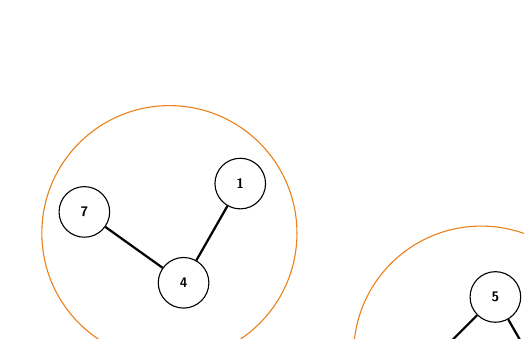
\begin{tikzpicture}[scale=1.8,auto,swap]

        \node[vertex] (1) at (-0.8,1.9) {1};
        \node[vertex] (2) at (3,1.7) {2};
        \node[vertex] (3) at (0.4,0.5) {3};
        \node[vertex] (4) at (-1.2,1.2) {4};
        \node[vertex] (5) at (1,1.1) {5};
        \node[vertex] (6) at (1.4,0.4) {6};
        \node[vertex] (7) at (-1.9,1.7) {7};

        \path[edge] (1) -- (4);
        \path[edge] (4) -- (7);
        \path[edge] (3) -- (5);
        \path[edge] (5) -- (6);
        \path[edge] (6) -- (3);

        \onslide<2->{
            \draw[color=vhilight] (-1.3,1.55) ellipse (0.9cm and 0.9cm);
            \draw[color=vhilight] (0.9,0.7) ellipse (0.9cm and 0.9cm);
            \draw[color=vhilight] (3,1.7) ellipse (0.3cm and 0.3cm);
        }

        \pgfresetboundingbox
        \path [use as bounding box] (-2.3,1.0) rectangle (1,3.0);
    \end{tikzpicture}
\end{frame}

\begin{frame}{Connected components}
    \vspace{30pt}
    \bi
        \item Also possible to find these components using depth-first search
        \item Pick some vertex we don't know anything about, and do a depth-first search from that vertex
        \item All vertices reachable from that starting vertex are in the same component
        \item Repeat this process until you have all the components
        \item Time complexity is $O(n + m)$
    \ei
\end{frame}

\begin{frame}[fragile]{Connected components}
    \begin{minted}[fontsize=\scriptsize]{cpp}
vector<int> adj[1000];
vector<int> component(1000, -1);

void find_component(int cur_comp, int u) {
    if (component[u] != -1) {
        return;
    }

    component[u] = cur_comp;

    for (int i = 0; i < adj[u].size(); i++) {
        int v = adj[u][i];
        find_component(cur_comp, v);
    }
}

int components = 0;
for (int u = 0; u < n; u++) {
    if (component[u] == -1) {
        find_component(components, u);
        components++;
    }
}
    \end{minted}
\end{frame}

\begin{frame}{Depth-first search tree}
    \vspace{30pt}

    \bi
        \item When we do a depth-first search from a certain vertex, the edges
            that we go over form a tree
        \item When we go from a vertex to another vertex that we haven't visited before, the edge that we take is called a \textit{forward edge}
        \item When we go from a vertex to another vertex that we've already visited before, the edge that we take is called a \textit{backward edge}
        \item To be more specific: the forward edges form a tree
        \vspace{20pt}
        \item \textit{see example}
    \ei
\end{frame}

\begin{frame}{Depth-first search tree}
    \vspace{30pt}

    \bi
        \item This tree of forward edges, along with the backward edges, can be analyzed to get a lot of information about the original graph
        \vspace{10pt}
        \item For example: a backward edge represents a cycle in the original graph
        \item If there are no backward edges, then there are no cycles in the original graph (i.e.\ the graph is acyclic)
    \ei
\end{frame}

\begin{frame}{Analyzing the DFS tree}
    \vspace{20pt}
    \bi
        \item Let's take a closer look at the depth-first search tree
        \vspace{10pt}
        \item First, let's number each of the vertices in the order that we visit them in the depth-first search
        \item For each vertex, we want to know the smallest number of a vertex that we reached when exploring the subtree rooted at the current vertex
        \vspace{10pt}
        \item Why? We'll see in a bit..
        \vspace{10pt}
        \item \textit{see example}
    \ei
\end{frame}

\begin{frame}[fragile]{Analyzing the DFS tree}
    \begin{minted}[fontsize=\scriptsize]{cpp}
const int n = 1000;
vector<int> adj[n];
vector<int> low(n), num(n, -1);
int curnum = 0;

void analyze(int u, int p) {
    low[u] = num[u] = curnum++;
    for (int i = 0; i < adj[u].size(); i++) {
        int v = adj[u][i];
        if (v == p) continue;
        if (num[v] == -1) {
            analyze(v, u);
            low[u] = min(low[u], low[v]);
        } else {
            low[u] = min(low[u], num[v]);
        }
    }
}

for (int u = 0; u < n; u++) {
    if (num[u] == -1) {
        analyze(u, -1);
    }
}
    \end{minted}
\end{frame}

\begin{frame}{Analyzing the DFS tree}
    \vspace{30pt}
    \bi
        \item Time complexity of this is just $O(n + m)$, since this is basically just one depth-first search
        \vspace{20pt}
        \item Now, as promised, let's see some applications of this
    \ei
\end{frame}

\begin{frame}{Bridges}
    \vspace{20pt}
    \bi
        \item We have a \textbf{connected undirected} graph
        \item Find an edge, so that if you remove that edge the graph is no longer connected
        \vspace{10pt}
        \item Naive algorithm: Try removing edges, one at a time, and find the connected components of the resulting graph
        \item That's pretty inefficient, $O(m(n + m))$
    \ei
\end{frame}

\begin{frame}{Bridges}
    \vspace{20pt}
    \bi
        \item Let's take a look at the values that we computed in the DFS tree
        \vspace{10pt}
        \item We see that a forward edge $(u,v)$ is a bridge if and only if \texttt{low[v]}>\texttt{num[u]}
        \vspace{10pt}
        \item Simple to extend our analyze function to return all bridges
        \item Again, this is just $O(n + m)$
    \ei
\end{frame}

\begin{frame}[fragile]{Bridges}
    \begin{minted}[fontsize=\tiny]{cpp}
const int n = 1000;
vector<int> adj[n];
vector<int> low(n), num(n, -1);
int curnum = 0;

vector<pair<int, int> > bridges;

void find_bridges(int u, int p) {
    low[u] = num[u] = curnum++;
    for (int i = 0; i < adj[u].size(); i++) {
        int v = adj[u][i];
        if (v == p) continue;
        if (num[v] == -1) {
            find_bridges(v, u);
            low[u] = min(low[u], low[v]);
        } else {
            low[u] = min(low[u], num[v]);
        }

        if (low[v] > num[u]) {
            bridges.push_back(make_pair(u, v));
        }
    }
}

for (int u = 0; u < n; u++) {
    if (num[u] == -1) {
        find_bridges(u, -1);
    }
}
    \end{minted}
\end{frame}

\begin{frame}{Strongly connected components}
    \vspace{10pt}
    \bi
        \item We know how to find connected components in undirected graphs
        \item But what about directed graphs?
        \vspace{10pt}
        \item Such components behave a bit differently in directed graphs, especially since if $v$ is reachable from $u$, it doesn't mean that $u$ is reachable from $v$
        \vspace{10pt}
        \item The definition remains the same, though
        \item A strongly connected component is a maximal subset of the vertices such that each pair of vertices is reachable from each other
    \ei
\end{frame}

\begin{frame}{Strongly connected components}
    \vspace{40pt}
    \bi
        \item The connected components algorithm won't work here
        \vspace{10pt}
        \item Instead we can use the depth-first search tree of the graph to find these components
        \vspace{10pt}
        \item \textit{see example}
    \ei
\end{frame}

\begin{frame}[fragile]{Strongly connected components}
    \begin{minted}[fontsize=\footnotesize]{cpp}
vector<int> adj[100];
vector<int> low(100), num(100, -1);
vector<bool> incomp(100, false);
int curnum = 0;

stack<int> comp;

void scc(int u) {

    // scc code...
}

for (int i = 0; i < n; i++) {
    if (num[i] == -1) {
        scc(i);
    }
}
    \end{minted}
\end{frame}

\begin{frame}[fragile]{Strongly connected components}
    \begin{minted}[fontsize=\tiny]{cpp}
void scc(int u) {

    comp.push(u);
    incomp[u] = true;

    low[u] = num[u] = curnum++;
    for (int i = 0; i < adj[u].size(); i++) {
        int v = adj[u][i];
        if (num[v] == -1) {
            scc(v);
            low[u] = min(low[u], low[v]);
        } else if (incomp[v]) {
            low[u] = min(low[u], num[v]);
        }
    }

    if (num[u] == low[u]) {
        printf("comp: ");
        while (true) {
            int cur = comp.top();
            comp.pop();
            incomp[cur] = false;
            printf("%d, ", cur);
            if (cur == u) {
                break;
            }
        }

        printf("\n");
    }
}
    \end{minted}
\end{frame}

\begin{frame}{Strongly connected components}
    \vspace{30pt}
    \bi
        \item Time complexity?
        \item Basically just the DFS analyze function (which was $O(n + m)$), with one additional loop to construct the component
        \item But each vertex is only in one component...
        \item Time complexity still just $O(n + m)$
    \ei
\end{frame}

% \begin{frame}{Example problem: Come and Go}
%     \bi
%         \item http://uva.onlinejudge.org/external/118/11838.html
%     \ei
% \end{frame}
\begin{frame}{Example problem: Tourist safety}
    Tourists sometimes like to explore the cities they're in. They start at
    their hotel, and then drive randomly around the city. This can be
    dangerous, however, as when the tourist becomes tired and wants to go home,
    it may not be possible!

    Given a directed road network, determine which road intersections are
    tourist-safe. A road intersection $u$ is tourist-safe if for each road
    intersection $v$ reachable from $u$, $u$ is reachable from $v$.
\end{frame}

\begin{frame}{Topological sort}
    \vspace{5pt}
    \bi
        \item We have $n$ tasks
        \item Each task $i$ has a list of tasks that must be completed before we can start task $i$
        \item Find an order in which we can process the tasks
        \vspace{5pt}
        \item Can be represented as a directed graph
            \bi
                \item Each task is a vertex in the graph
                \item If task $j$ should be finished before task $i$, then we add a directed edge from vertex $i$ to vertex $j$
            \ei
        \vspace{5pt}
        \item Notice that this can't be solved if the graph contains a cycle
        \vspace{5pt}
        \item A modified depth-first search can be used to find an ordering in $O(n + m)$ time, or determine that one does not exist
    \ei
\end{frame}

\begin{frame}[fragile]{Topological sort}
    \begin{minted}[fontsize=\scriptsize]{cpp}
vector<int> adj[1000];
vector<bool> visited(1000, false);
vector<int> order;

void topsort(int u) {
    if (visited[u]) {
        return;
    }

    visited[u] = true;
    for (int i = 0; i < adj[u].size(); i++) {
        int v = adj[u][i];
        topsort(v);
    }

    order.push_back(u);
}

for (int u = 0; u < n; u++) {
    topsort(u);
}
    \end{minted}
\end{frame}

% \begin{frame}{Example problem: Ordering Tasks}
%     \bi
%         \item http://uva.onlinejudge.org/external/103/10305.html
%     \ei
% \end{frame}

\begin{frame}{Breadth-first search}
    \vspace{30pt}
    \bi
        \item There's another search algorithm called Breadth-first search
        \item Only difference is the order in which it visits the vertices
        \item It goes in order of increasing distance from the source vertex
    \ei
\end{frame}


\begin{frame}{Breadth-first search}
  \begin{figure}
    \begin{tikzpicture}[auto, swap]
      \node[vertex] (0) at (-0.3,2) {0};
      \node[vertex] (1) at (0.0,-0.5) {1};
      \node[vertex] (2) at (1.9,0.7) {2};
      \node[vertex] (3) at (2.4,2.7) {3};
      \node[vertex] (4) at (3.4,-0.8) {4};
      \node[vertex] (5) at (3.9,1) {5};
      \node[vertex] (6) at (6.2,1.1) {6};
      \node[vertex] (7) at (6.1,-0.9) {7};
      \node[vertex] (8) at (5.7,3.2) {8};
      \node[vertex] (9) at (8.3,2.1) {9};
      \node[vertex] (10) at (8.1,0.1) {10};

      \path[dedge] (0) -- (1);
      \path[dedge] (0) -- (2);

      \path[dedge] (1) -- (4);

      \path[dedge] (2) -- (1);
      \path[dedge] (2) -- (3);

      \path[dedge] (3) -- (0);

      \path[dedge] (4) -- (5);

      \path[dedge] (5) -- (2);
      \path[dedge] (5) -- (3);
      \path[dedge] (5) -- (6);
      \path[dedge] (5) -- (7);
      \path[dedge] (5) -- (8);

      %\path[dedge] (6) -- (5);
      \path[dedge] (6) -- (8);
      \path[dedge] (6) -- (7);

      %\path[dedge] (8) -- (5);
      \path[dedge] (8) to [bend left] (9);

      \path[dedge] (9) to [bend left] (8);

      \path[dedge] (7) -- (10);

      \only<2-4>{\node[vertex,fill=vhilight] (0) at (-0.3,2) {0};}
      \only<3-4>{
        \path[dedge,vhilight] (0) -- (1);
        \path[dedge,vhilight] (0) -- (2);
      }

      \only<5->{\node[vertex,fill=title] (0) at (0) {0};}
      \only<5->{\path[dedge,thick,title] (0) -- (1);}
      \only<5->{\path[dedge,thick,title] (0) -- (2);}
      \only<5->{\node[vertex,fill=vhilight] (1) at (1) {1};}

      \only<6-7>{\path[dedge,vhilight] (1) -- (4);}
      \only<8->{\path[dedge,thick,title] (1) -- (4);}

      \only<8->{\node[vertex,fill=title] (1) at (1) {1};}
      \only<8-10>{\node[vertex,fill=vhilight] (2) at (2) {2};}
      \only<9-10>{\path[dedge,vhilight] (2) -- (3);}
      \only<8-10>{\node[vertex,fill=vhilight] (2) at (2) {2};}


      \only<10>{\path[dedge,vhilight] (2) -- (3);}
      \only<11->{\node[vertex,fill=title] (2) at (2) {2};}
      \only<11->{\path[dedge,title,thick] (2) -- (3);}
      \only<11-13>{\node[vertex,fill=vhilight] (4) at (4) {4};}
      \only<12-13>{\path[dedge,vhilight] (4) -- (5);}

      \only<14->{\node[vertex,fill=title] (4) at (4) {4};}
      \only<14->{\path[dedge,thick,title] (4) -- (5);}
      \only<14>{\node[vertex,fill=vhilight] (3) at (3) {3};}

      \only<14>{\node[vertex,fill=vhilight] (3) at (3) {3};}
      \only<15->{\node[vertex,fill=title] (3) at (3) {3};}

      \only<15-17>{\node[vertex,fill=vhilight] (5) at (5) {5};}
      \only<16-17>{
        \path[dedge,vhilight] (5) -- (6);
        \path[dedge,vhilight] (5) -- (7);
        \path[dedge,vhilight] (5) -- (8);
      }
      \only<18->{
        \node[vertex,fill=title] (5) at (5) {5};
        \path[dedge,title,thick] (5) -- (6);
        \path[dedge,title,thick] (5) -- (7);
        \path[dedge,title,thick] (5) -- (8);
      }
      \only<18>{ \node[vertex,fill=vhilight] (6) at (6) {6}; }
      \only<19->{ \node[vertex,fill=title] (6) at (6) {6}; }

      \only<19-21>{ \node[vertex,fill=vhilight] (7) at (7) {7}; }
      \only<20-21>{\path[dedge,vhilight] (7) -- (10);}

      \only<22->{ 
        \node[vertex,fill=title] (7) at (7) {7};
        \path[dedge,title,thick] (7) -- (10);
      }

      \only<22-24>{\node[vertex,fill=vhilight] (8) at (8) {8};}
      \only<23-24>{\path[dedge,vhilight] (8) to[bend left] (9)};

      \only<25->{
        \node[vertex,fill=title] (8) at (8) {8};
        \path[dedge,title] (8) to[bend left] (9);
      }
      \only<25>{\node[vertex,fill=vhilight] (10) at (10) {10};}
      \only<26->{\node[vertex,fill=title] (10) at (10) {10};}
      \only<26>{\node[vertex,fill=vhilight] (9) at (9) {9};}
      \only<27->{\node[vertex,fill=title] (9) at (9) {9};}

    \end{tikzpicture}
  \end{figure}

  %\mintinline{cpp}{Queue: }
  \texttt{ \begin{tabular}{l l}
  \texttt{Queue: } & 
   \only<2-3>{{\color{vhilight}0}}\only<4>{{\color{vhilight}0} 1 2}\only<5-6>{{\color{vhilight}1} 2}\only<7>{{\color{vhilight}1} 2 4}\only<8-9>{{\color{vhilight}2} 4}\only<10>{{\color{vhilight}2} 4 3}\only<11-12>{{\color{vhilight}4} 3}\only<13>{{\color{vhilight}4} 3 5}\only<14>{{\color{vhilight}3} 5}\only<15-16>{{\color{vhilight}5}}\only<17>{{\color{vhilight}5} 6 7 8}\only<18>{{\color{vhilight}6} 7 8}\only<19-20>{{\color{vhilight}7} 8}\only<21>{{\color{vhilight}7} 8 10}\only<22-23>{{\color{vhilight}8} 10}\only<24>{{\color{vhilight}8} 10 9}\only<25>{{\color{vhilight}10} 9}\only<26>{{\color{vhilight}9}}
  \end{tabular}}

  \vspace{10pt}
  \texttt{
    \begin{tabular}{l | c c c c c c c c c c c }
      & 0 & 1 & 2 & 3 & 4 & 5 & 6 & 7 & 8 & 9 & 10 \\
      marked 
      & \only<1>{0}\only<2->{{\color{title}1}} 
      & \only<1-3>{0}\only<4->{{\color{title}1}} 
      & \only<1-3>{0}\only<4->{{\color{title}1}} 
      & \only<1-9>{0}\only<10->{{\color{title}1}} 
      & \only<1-6>{0}\only<7->{{\color{title}1}} 
      & \only<1-12>{0}\only<13->{{\color{title}1}} 
      & \only<1-16>{0}\only<17->{{\color{title}1}} 
      & \only<1-16>{0}\only<17->{{\color{title}1}} 
      & \only<1-16>{0}\only<17->{{\color{title}1}} 
      & \only<1-23>{0}\only<24->{{\color{title}1}}
      & \only<1-20>{0}\only<21->{{\color{title}1}} \\
    \end{tabular}}
\end{frame}

\begin{frame}[fragile]{Breadth-first search}
    \begin{minted}[fontsize=\footnotesize]{cpp}
vector<int> adj[1000];
vector<bool> visited(1000, false);

queue<int> Q;
Q.push(start);
visited[start] = true;

while (!Q.empty()) {
    int u = Q.front(); Q.pop();

    for (int i = 0; i < adj[u].size(); i++) {
        int v = adj[u][i];
        if (!visited[v]) {
            Q.push(v);
            visited[v] = true;
        }
    }
}
    \end{minted}
\end{frame}

\begin{frame}{Shortest path in unweighted graphs}
    \vspace{5pt}
    \bi
        \item We have an unweighted graph, and want to find the shortest path from $A$ to $B$
        \item That is, we want to find a path from $A$ to $B$ with the minimum number of edges
        \vspace{10pt}
        \item Breadth-first search goes through the vertices in increasing order of distance from the start vertex
        \item Just do a single breadth-first search from $A$, until we find $B$
        \vspace{5pt}
        \item Or let the search continue through the whole graph, and then we have the shortest paths from $A$ to all other vertices
        \item Shortest path from $A$ to all other vertices: $O(n + m)$
    \ei
\end{frame}

\begin{frame}[fragile]{Shortest path in unweighted graphs}

    \begin{minted}[fontsize=\scriptsize]{cpp}
vector<int> adj[1000];
vector<int> dist(1000, -1);

queue<int> Q;
Q.push(A);
dist[A] = 0;

while (!Q.empty()) {
    int u = Q.front(); Q.pop();

    for (int i = 0; i < adj[u].size(); i++) {
        int v = adj[u][i];
        if (dist[v] == -1) {
            Q.push(v);
            dist[v] = 1 + dist[u];
        }
    }
}

printf("%d\n", dist[B]);
    \end{minted}

\end{frame}

% TODO: Reconstructing the shortest path

% TODO: Example problem

\end{document}

